\documentclass[final]{beamer}
%% Possible paper sizes: a0, a0b, a1, a2, a3, a4.
%% Possible orientations: portrait, landscape
%% Font sizes can be changed using the scale option.
\usepackage[size=a0,orientation=portrait,scale=1.1]{beamerposter}

\usetheme{gemini}
\usecolortheme{seagull}
\useinnertheme{rectangles}

% ====================
% Packages
% ====================

\usepackage[utf8]{inputenc}
\usepackage{graphicx}
\usepackage{booktabs}
\usepackage{tikz}
\usepackage{pgfplots}

% ====================
% Lengths
% ====================

% If you have N columns, choose \sepwidth and \colwidth such that
% (N+1)*\sepwidth + N*\colwidth = \paperwidth
\newlength{\sepwidth}
\newlength{\colwidth}
\setlength{\sepwidth}{0.03\paperwidth}
\setlength{\colwidth}{0.45\paperwidth}

\newcommand{\separatorcolumn}{\begin{column}{\sepwidth}\end{column}}

% ====================
% Logo (optional)
% ====================

% LaTeX logo taken from https://commons.wikimedia.org/wiki/File:LaTeX_logo.svg
% use this to include logos on the left and/or right side of the header:
\logoright{
\includegraphics[height=12cm]{logos/WSAI_Logo_new.png}}
\logoleft{
\includegraphics[height=10cm]{logos/IIT_Madras_Logo.svg.png}}

% ====================
% Footer (optional)
% ====================

\footercontent{
	Indian Institute of Technology, Madras, India \hfill
	\insertdate \hfill
	\href{mailto:me21b174@smail.iitm.ac.in}{\texttt{me21b174@smail.iitm.ac.in}}
}
% (can be left out to remove footer)

% ====================
% My own customization
% - BibLaTeX
% - Boxes with tcolorbox
% - User-defined commands
% ====================
\input{custom-defs.tex}

%% Reference Sources
\addbibresource{refs.bib}
\renewcommand{\pgfuseimage}[1]{\includegraphics[scale=2.0]{#1}}

\title{Digital Twin - Based Multi Echelon Inventory Optimization}%project/6450fb59b06eb1a2f0ba8b8e

\author{Sakthe Balan G K}

\institute[shortinst]{Indian Institute of Technology, Madras, India}

\date{January 31, 2026}

\begin{document}
	
\begin{frame}[t]
	
	\begin{columns}[t]
	
	\begin{column}{2\colwidth+\sepwidth}
	\vspace{-3em}
	% \begin{block}{Introduction}

	% 	Inventory management decisions play a central role in determining the efficiency, resilience, and cost-effectiveness of modern supply chains. 
	% 	Organizations operating multi-echelon inventory networks must make critical inventory and replenishment decisions under demand uncertainty, transportation limitations, and operational constraints, often without clear visibility into their system-wide consequences. 
	% 	As a result, changing inventory policies in real-world systems is inherently risky, since decision-makers often lack the ability to anticipate impacts on downstream service levels, costs, and overall system stability.
	% 	\vspace{0.5em}

	% 	Despite extensive research in \textbf{Multi-Echelon Inventory Optimization (MEIO)}, a substantial gap remains between theoretical models and practical deployment. 
	% 	Classical MEIO approaches rely on strong assumptions such as stationary demand, simplified cost structures, and unconstrained transportation, which limit their applicability to realistic supply chains. 
	% 	More recent research has explored simulation-based optimization, deep reinforcement learning, and data-driven digital twin approaches. 
	% 	While these methods offer greater modeling flexibility, they typically require a reliable and validated simulation environment, which is often proprietary, domain-specific, or unavailable as an open source model.
	% 	\vspace{0.5em}

	% 	Consequently, many organizations hesitate to experiment with alternative inventory policies or forecasting strategies, as the outcomes of such changes are difficult to evaluate safely. 
	% 	There is a clear need for a \textbf{modular, transparent, and extensible framework} that enables decision-makers to simulate supply chain behavior using historical and real-time data, assess performance under uncertainty, and explore policy alternatives prior to real-world deployment.
	% 	\vspace{0.5em}

	% 	This work addresses this gap by developing a \textbf{Digital Twin–Based Simulator} for multi-echelon inventory systems with explicit modeling of stochastic demand, transportation capacity constraints, and cost components. 
	% 	The current phase focuses on building and validating the core simulation modules and their interactions to ensure realistic system behavior. 
	% 	Building on this validated foundation, the framework is designed to support future inventory optimization studies, including the impact of demand forecasting accuracy on policy selection, transportation policy evaluation, cost–service trade-offs, and learning-based inventory control strategies.

	% \end{block}

	\begin{block}{Introduction}
		\textbf{Background and Motivation}  

		Inventory management decisions play a central role in determining the efficiency, resilience, and cost-effectiveness of 
		modern supply chains. Organizations operating multi-echelon inventory networks must make critical replenishment 
		decisions under demand uncertainty, transportation limitations, and operational constraints, often without clear 
		visibility into system-wide consequences. As a result, modifying inventory policies in real-world systems is inherently
		risky, since downstream impacts on service levels, costs, and stability are difficult to anticipate in advance.

		\vspace{0.4em}

		While a wide range of analytical models exist for multi-echelon inventory systems,
		their assumptions often simplify demand dynamics, transportation constraints, or
		network structure. In practice, decision-makers frequently rely on simulation tools
		to evaluate inventory policies and operational scenarios before deployment. However,
		many such tools are proprietary, domain-specific, or tightly coupled to specific
		industrial settings, limiting their transparency and extensibility.

		\vspace{0.4em}

		\textbf{Key contribution}  

		This work addresses this gap by developing a \textbf{digital twin-based simulator} for multi-echelon inventory 
		systems with explicit modeling of stochastic demand, transportation capacity constraints, and cost components. 
		The current phase focuses on building and validating the core simulation modules and their interactions to ensure 
		realistic system behavior. The framework is designed to be \textbf{modular, extensible and open source}, serving as a foundation
		for future studies on inventory optimization including the impact of demand forecasting on policy selection,
		transportation policy evaluation and cost-service trade-offs.

	\end{block}



	\end{column}

	\end{columns}

	\begin{columns}[t]
		\separatorcolumn
		
		\begin{column}{\colwidth}
			
			\begin{block}{Data}

			\begin{itemize}
				\item \textbf{Demand Data:}  
				Retail-level demand is provided either as generated time-series or as processed data derived from the M5 forecasting dataset (Walmart sales data).

				\item \textbf{Inventory Data:}  
				Initial inventory levels, storage capacities, and replenishment parameters are defined for each echelon of the supply chain.

				\item \textbf{Transportation Data:}  
				Transportation links are defined through route connectivity, capacity constraints, and lead times governing material flow between echelons.

				\item \textbf{Cost Parameters:}  
				Holding costs, stockout penalties, and transportation costs are specified to evaluate cost–service trade-offs.
			\end{itemize}

			\vspace{0.4em}
			Non-demand parameters are defined to enable systematic testing and validation. The simulator is designed to directly take in real-world operational inputs without changes to the simulation logic.

			\end{block}



			\begin{block}{System Architecture and Simulator Design}

			The digital twin represents a multi-echelon supply chain as a directed network of inventory-holding nodes 
			(supplier, warehouse, retailer) connected by transportation links with finite capacity and lead times. 
			Each node maintains a local inventory state, while transportation links explicitly govern feasible material
			flow between echelons.

			\vspace{0.4em}

			\textbf{Discrete-Time Simulation Flow of the Digital Twin}
			\vspace{0.4em}

			\begin{center}
			\begin{minipage}{0.95\linewidth}
			\centering
			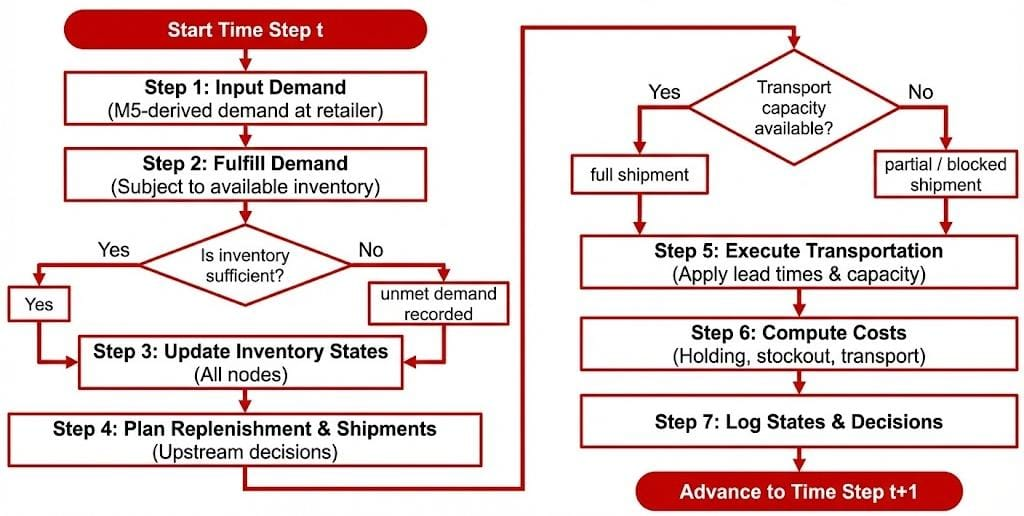
\includegraphics[scale = 0.85]{flowchart.jpeg}
			\end{minipage}
			\end{center}

			\vspace{0.4em}

			\textbf{Simulator Features}

			\begin{itemize}

				\item \textbf{Flexible Input Interface:}  
				The simulator accepts structured inputs via CSV configuration files or as deterministic parameter 
				definitions in json, enabling easy switching between experimental setups and real-world data sources.

				\item \textbf{Multi-Echelon and Multi-Route Modeling:}  
				Arbitrary supply chain topologies are supported, including one-many, many-one and many-many connections 
				between nodes and multiple tranportation routes between the same 
				pair of nodes with independent capacities and lead times.

				\item \textbf{Inventory Policy Support:}  
				Each inventory-holding node applies a configurable replenishment policy. The current implementation 
				supports base-stock and $(s, S)$ - type policies, with a modular design for extending to additional policies.

				\item \textbf{SKU-Level Extensibility:}  
				The simulator is designed to support both single-SKU experiments and extension to multiple SKUs without 
				changes to the core execution logic.

				\item \textbf{Shipment Planning and Execution:}  
				Replenishment decisions generate shipment requests that are executed subject to transportation feasibility, 
				allowing partial or blocked shipments and realistic delay propagation - modifyable by changing the tranportation policy.
			
			\end{itemize}

			\end{block}


			



				
			\begin{block}{Results}

				\textbf{Simulator Validation and Demand Shock Analysis}
				\begin{itemize}
					\item \textbf{Constant-demand validation (Fig.~a):}  
					A simple three-echelon  1 Supplier - 1 Warehouse - 1 Retailer network is simulated with an infinite-supply source and base-stock policies.
					Retailer demand is fixed at 5 units/day with constant lead times (2 and 1 days), and inventory position is plotted.

					\item \textbf{Demand shock experiment (Fig.~b):}  
					Using the same network and policy, a one-day demand spike of 20 units is introduced at the retailer.
					On-hand inventory is plotted to observe the delayed upstream response caused by lead times and 
					transportation constraints.
				\end{itemize}

				\vspace{0.8em}

				\begin{columns}[t]
					\begin{column}{0.48\linewidth}
						\centering
						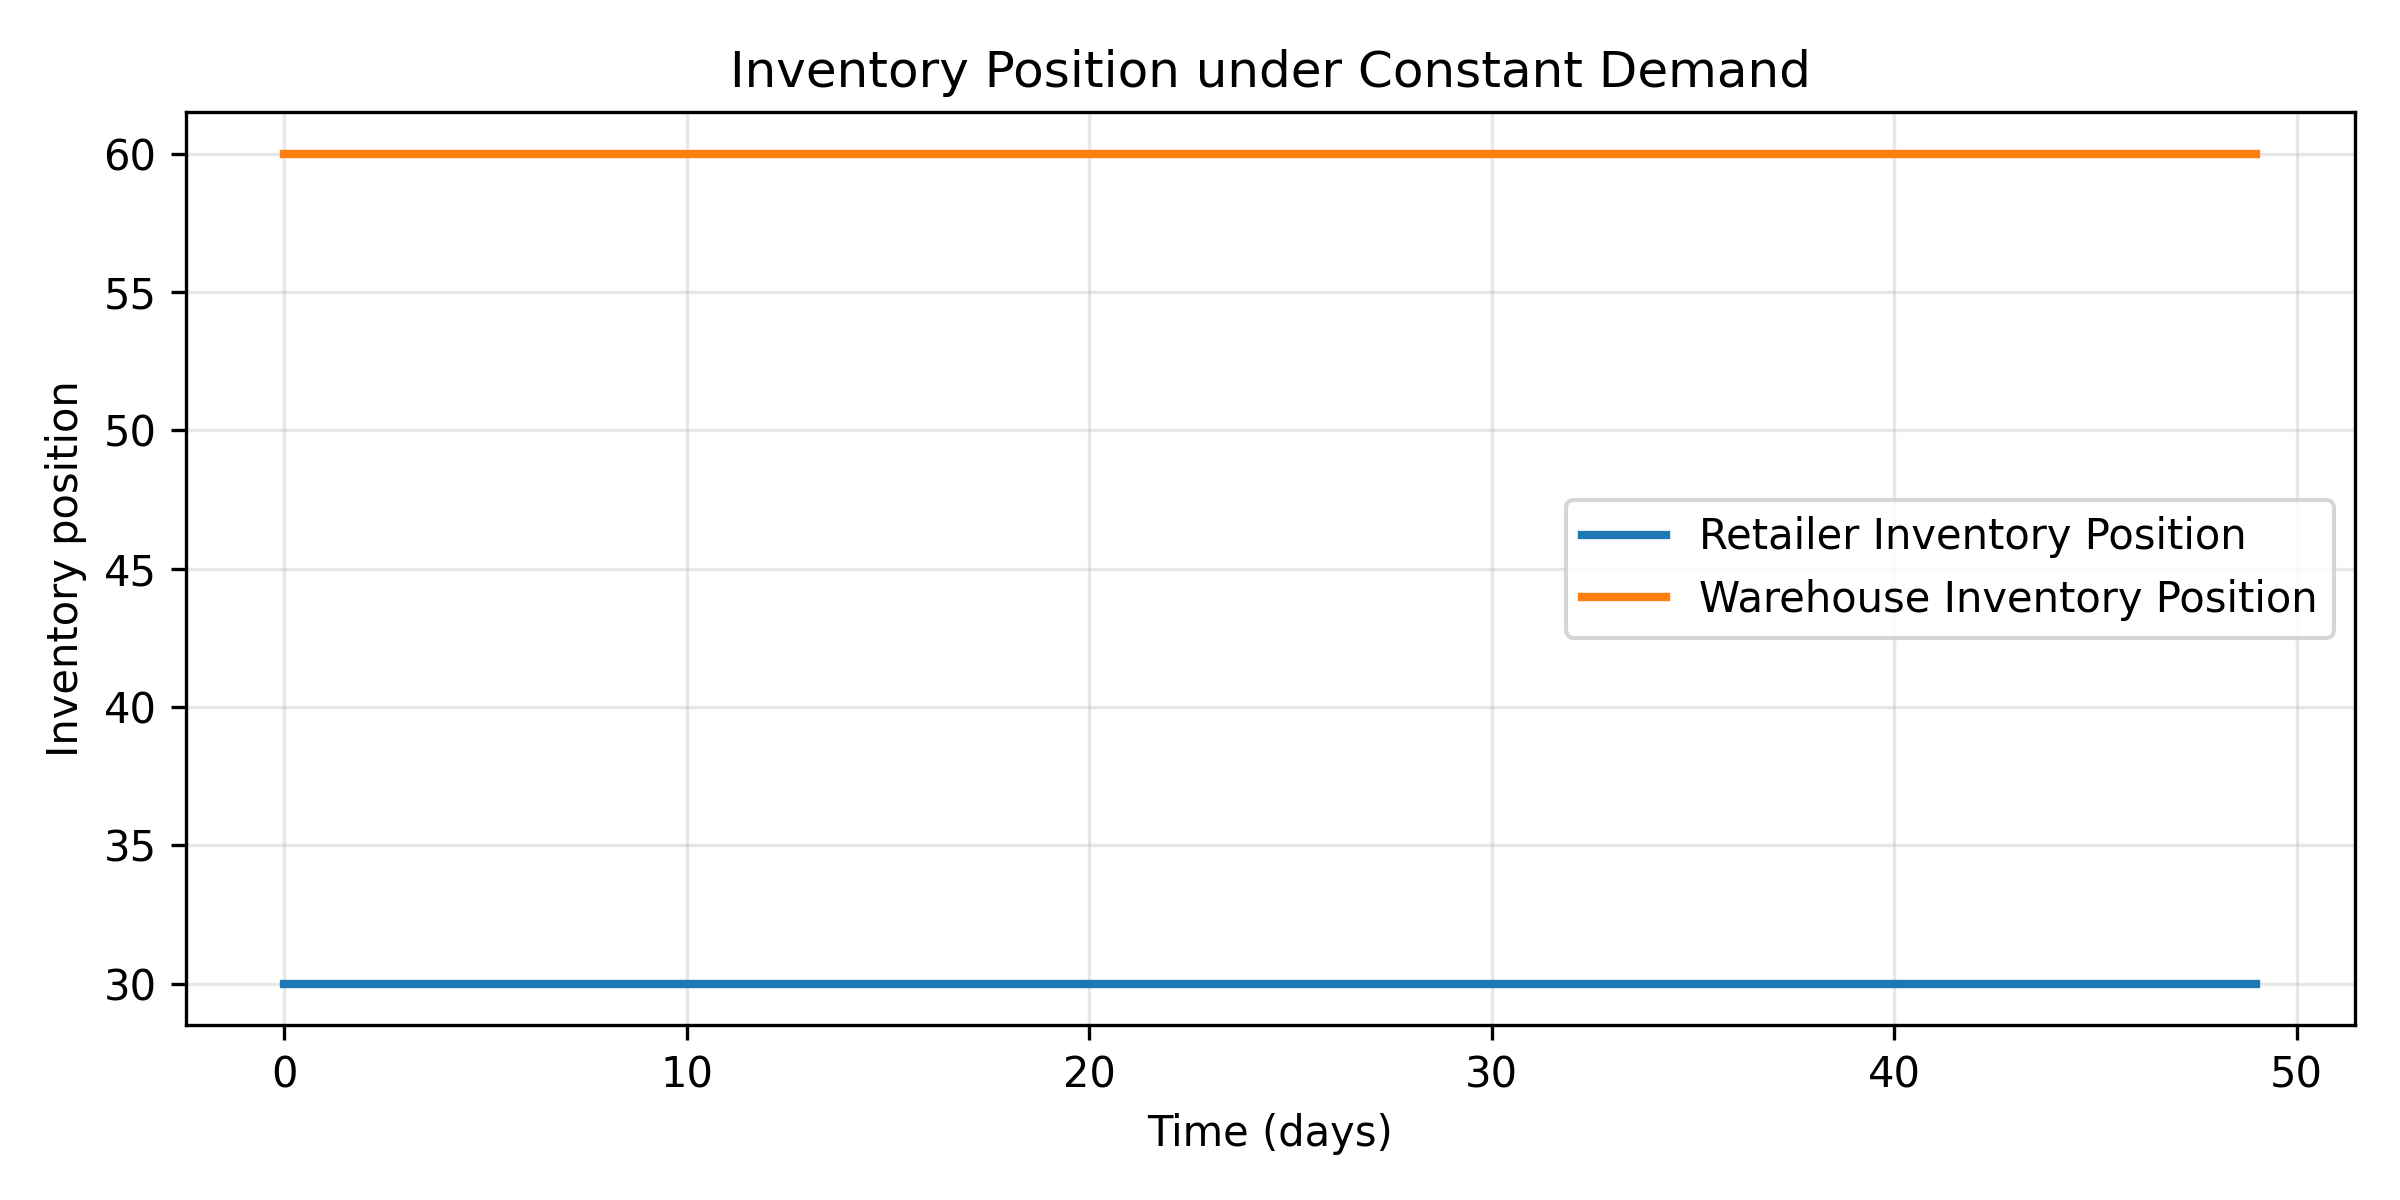
\includegraphics[scale = 0.8]{ip_constant.png}
						
						\vspace{0.3em}
						(a) Inventory Position under Constant Demand
						
					\end{column}

					\hfill

					\begin{column}{0.48\linewidth}
						\centering
						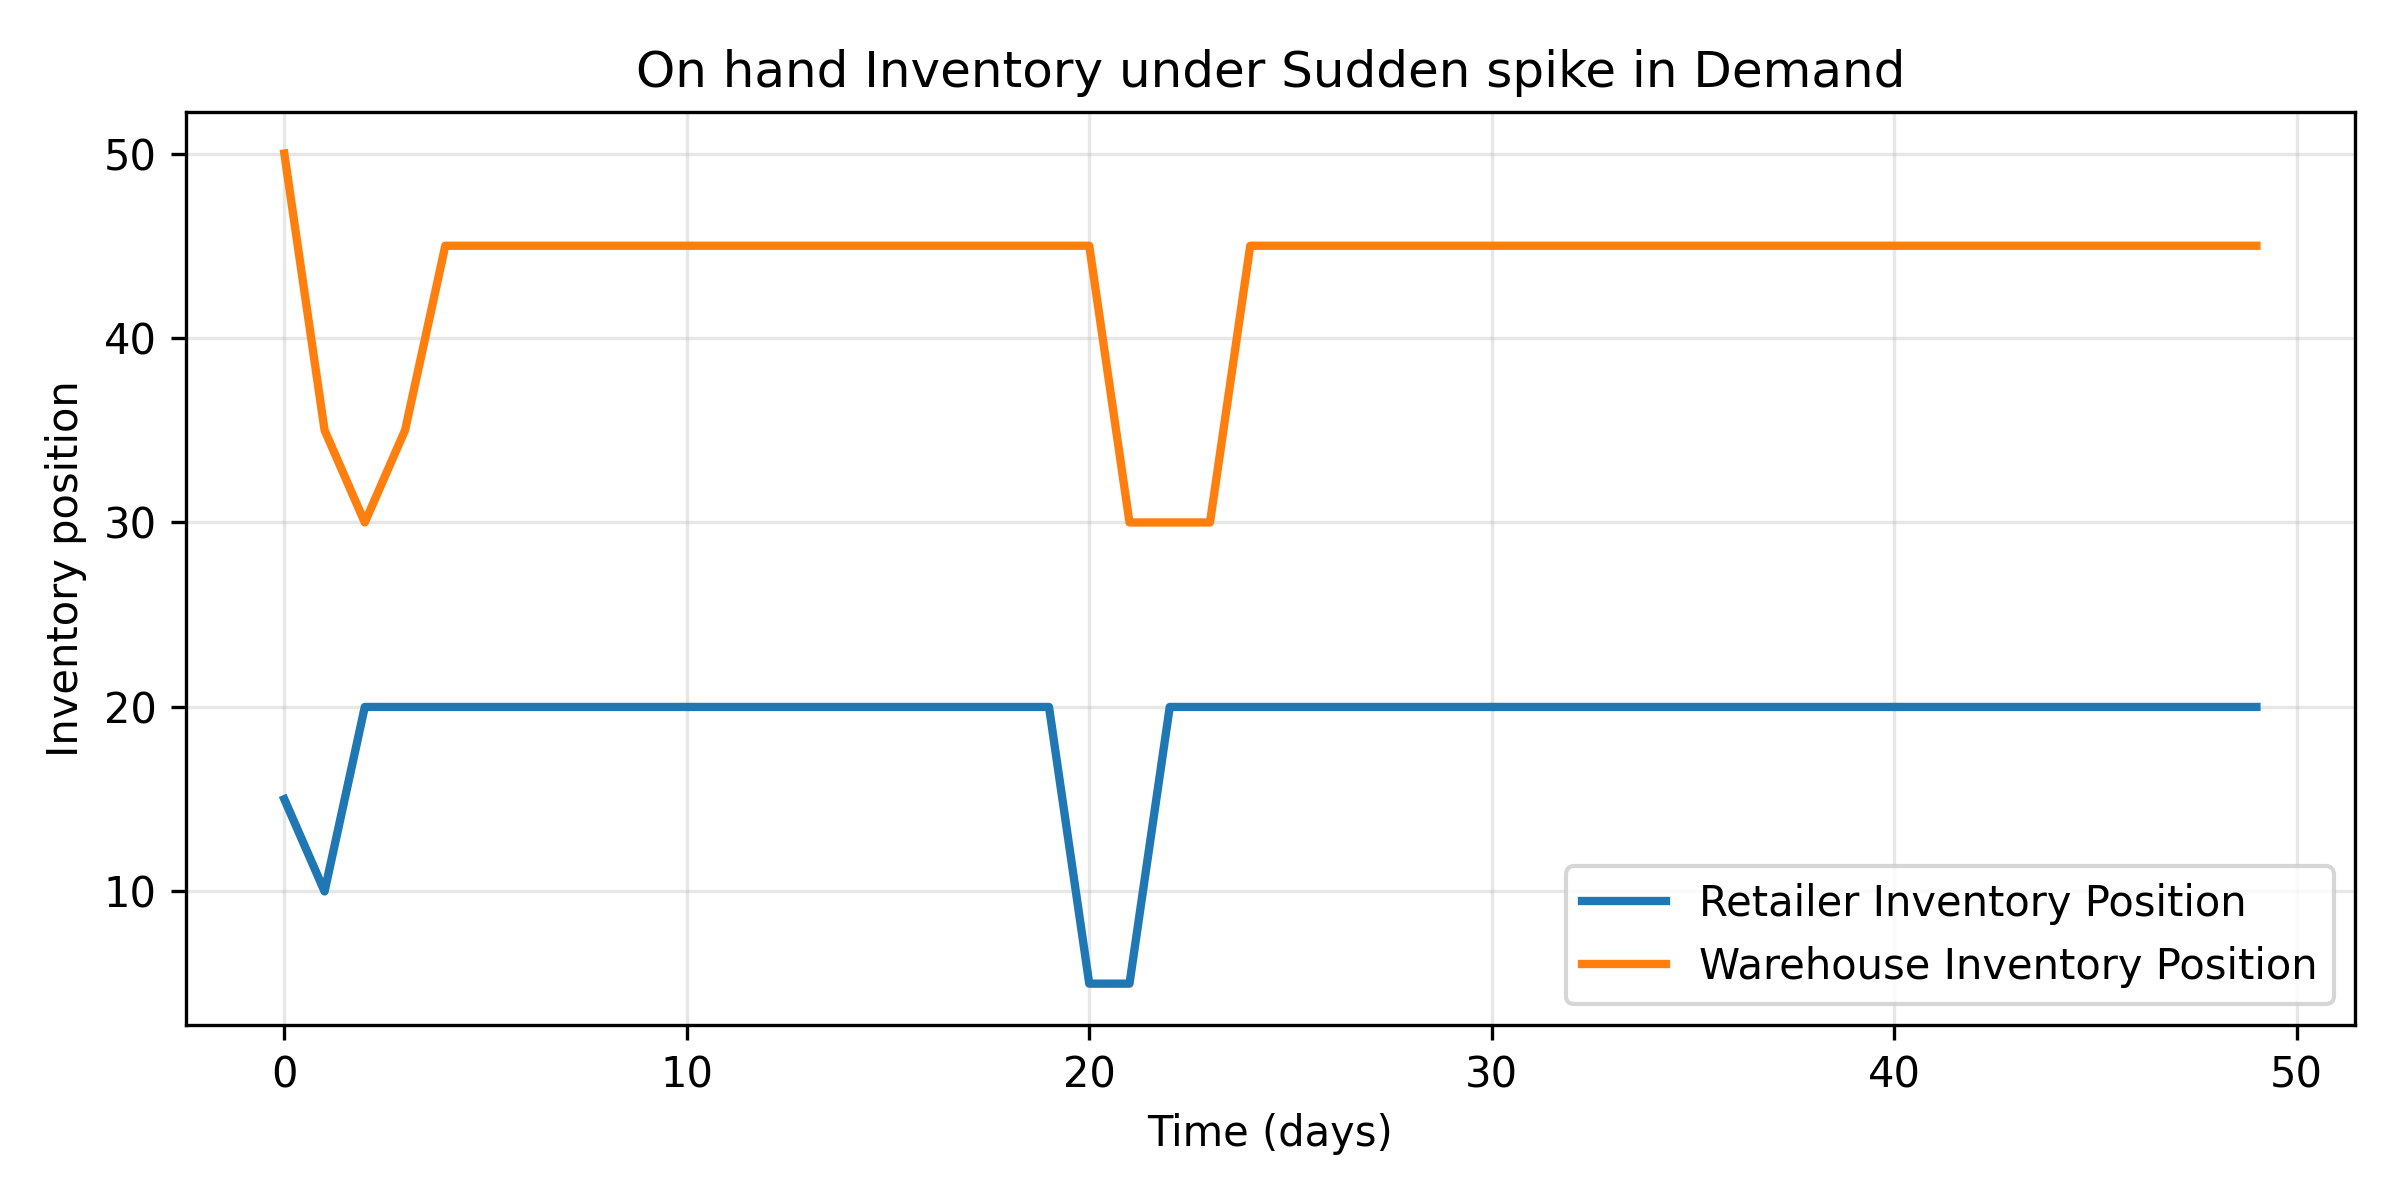
\includegraphics[scale = 0.8]{onhand_inventory_spike.png}
						
						\vspace{0.3em}
						(b) On-hand Inventory under Demand Spike
						
					\end{column}
				\end{columns}

			\end{block}

		\end{column}
	
		\separatorcolumn
		
		\begin{column}{\colwidth}
			
			\begin{block}{Results}

				\begin{itemize}
					\item Under constant demand, the inventory position at both the retailer and warehouse
					remains regulated at the base-stock level, validating the ordering and pipeline logic.

					\item When a demand spike is introduced, inventory position remains regulated due to
					policy response, while on-hand inventory shows an initial transient dip due to system
					warm-up, followed by an immediate retailer dip and a delayed warehouse response caused
					by lead times.
				\end{itemize}

				\vspace{0.5em}

				% \textbf{Inventory Position Definition}
				% \vspace{-0.3em}
				% \[
				% \text{Inventory Position}
				% =
				% \text{On-hand Inventory}
				% +
				% \text{Pipeline Inventory}
				% +
				% \text{Placed Orders}
				% -
				% \text{Backorders}
				% \]

				% \noindent
				\textbf{Policy and Transport Constraints Analysis}

				We compare \textbf{base-stock} and \textbf{(s,S)} policies on the 
				\textbf{same three-echelon synthetic network} used in 
				Fig.~(a) and Fig.~(b). In an (s, S) policy, replenishment is triggered only when inventory falls below a 
				reorder point s, and orders raise inventory up to a target level S. Only warehouse policy and 
				transportation capacity of a single link (warehouse to retailer) are varied.

				\vspace{0.8em}
				\begin{columns}[t]
					\begin{column}{0.48\linewidth}
						\centering
						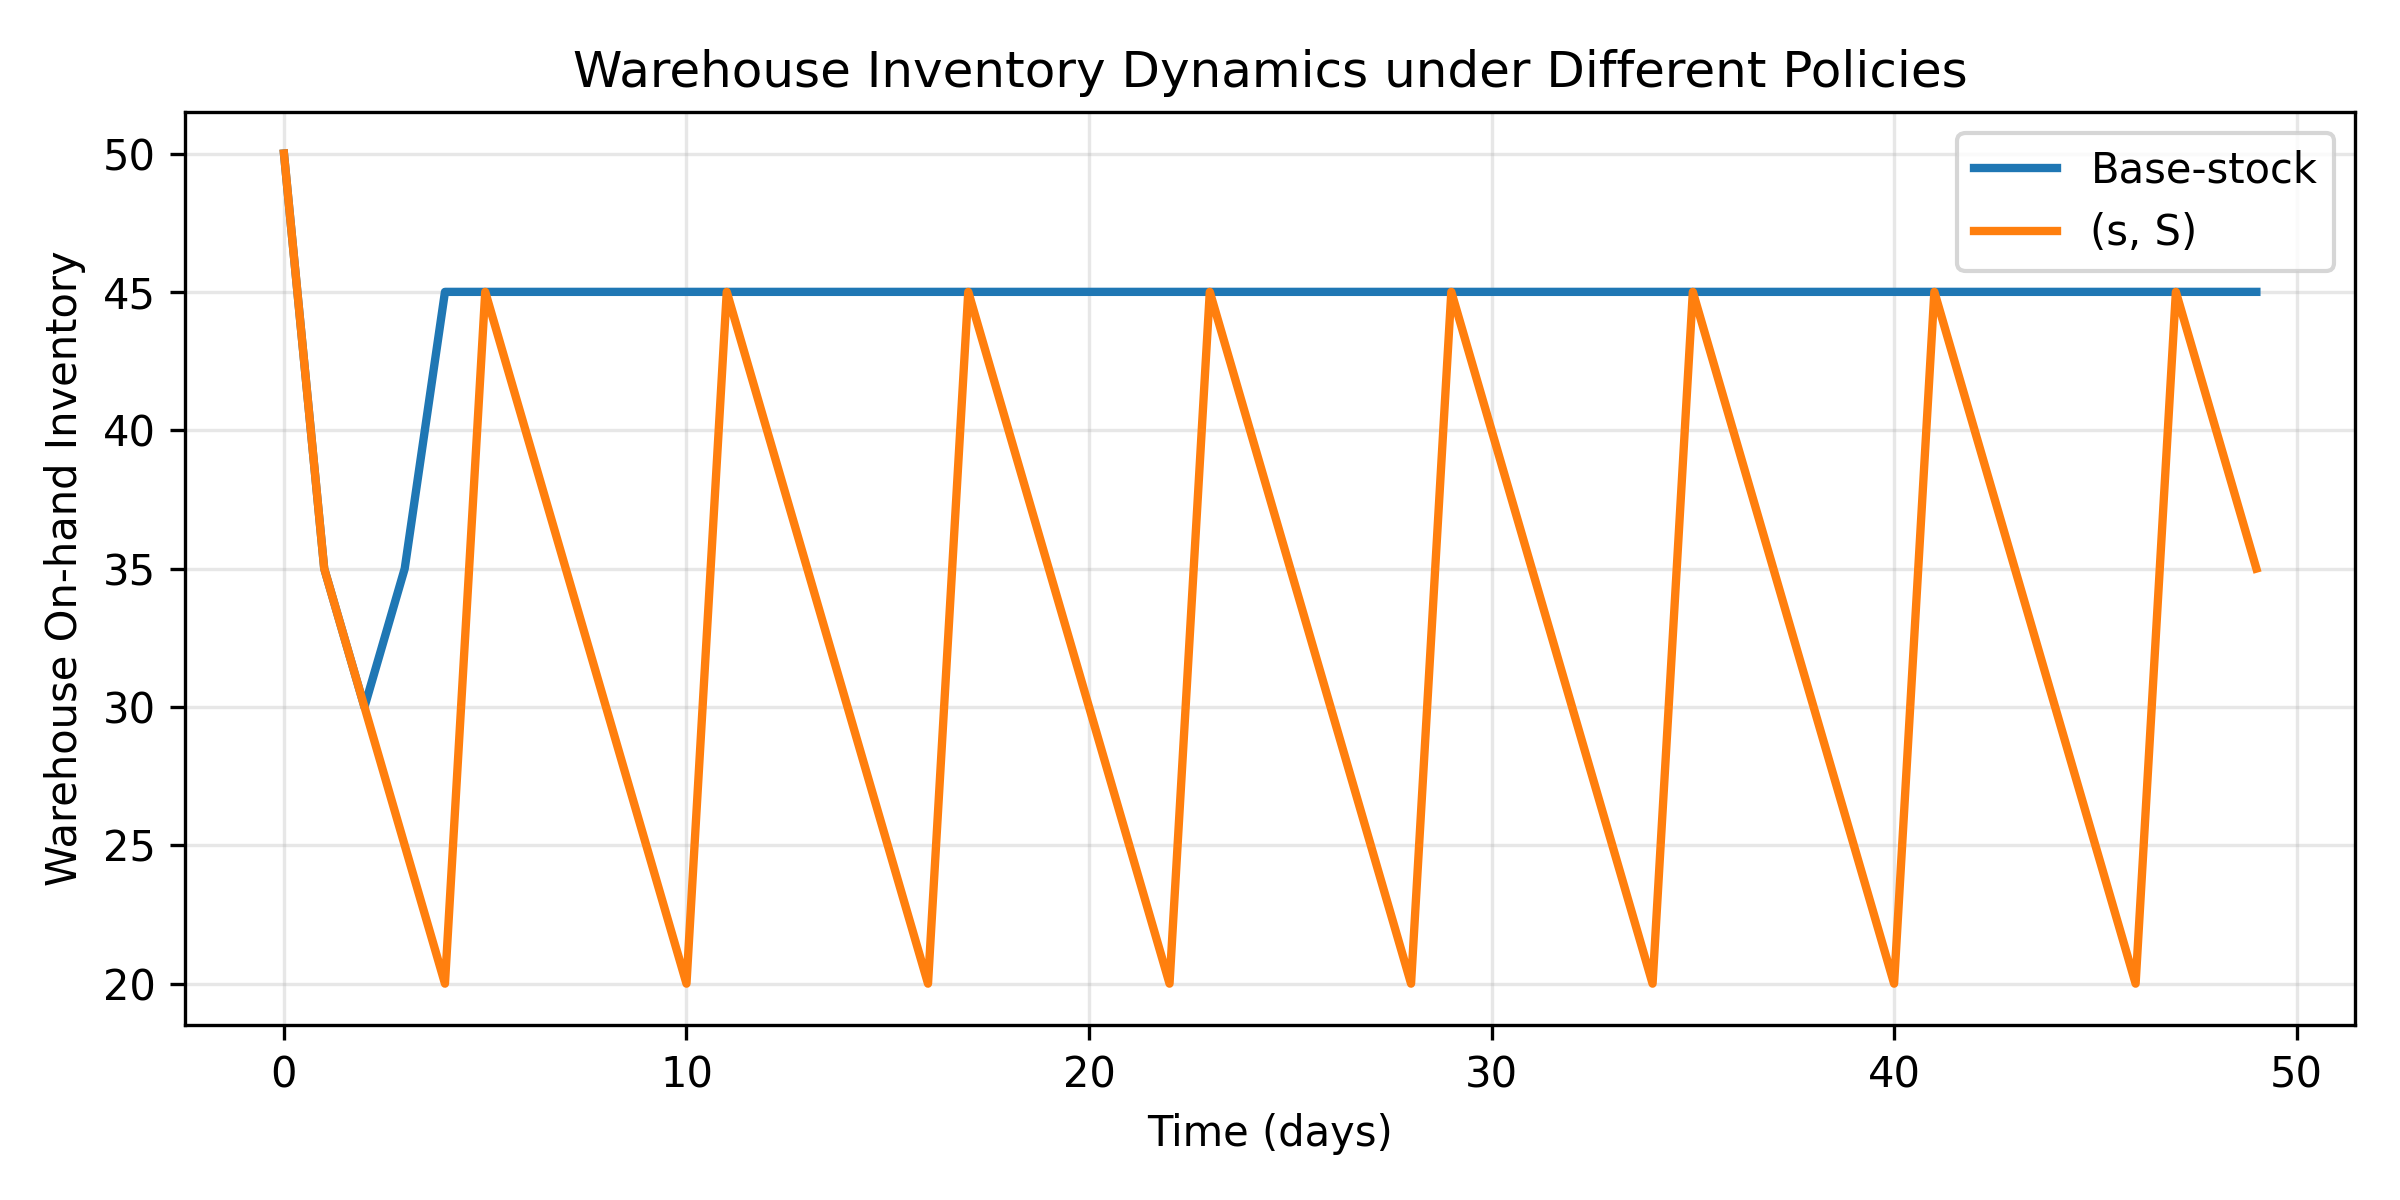
\includegraphics[scale = 0.8]{2_policy_without.png}
						
						\vspace{0.3em}
						(c) Warehouse inventory without transport delay
						
					\end{column}

					\hfill

					\begin{column}{0.48\linewidth}
						\centering
						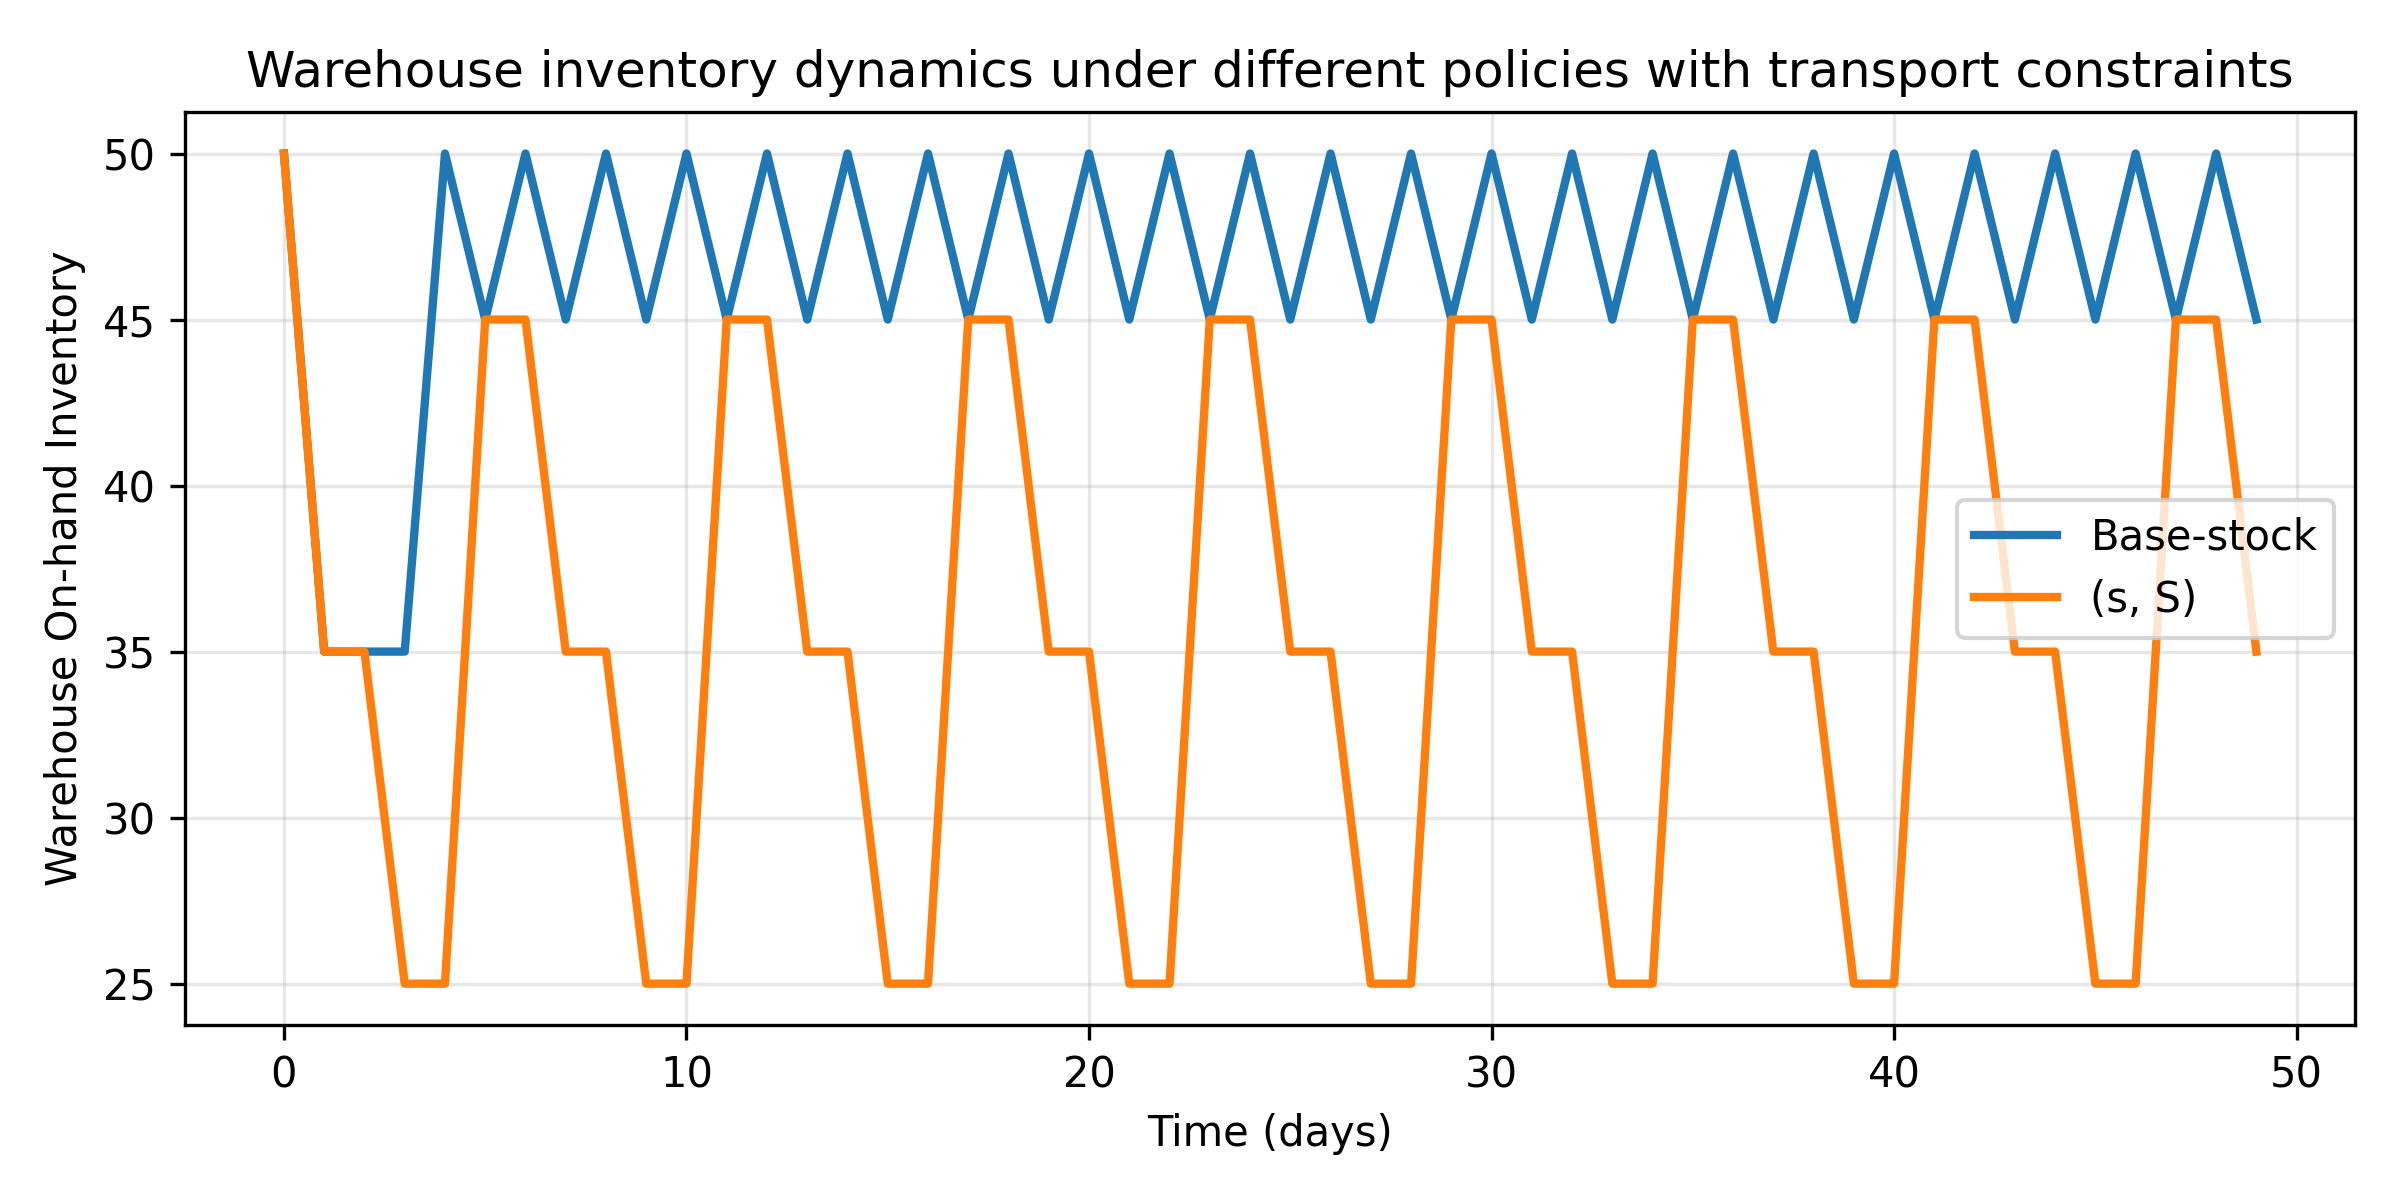
\includegraphics[scale = 0.8]{2_policy_with.png}
						
						\vspace{0.3em}
						(d) Warehouse inventory with transport delay
						
					\end{column}
				\end{columns}
				
				\vspace{0.5em} 

				\begin{itemize}
					\item \textbf{Without transport constraints (Fig. c):}  
					Base-stock stabilizes at an on-hand level of $45$, corresponding to a target of $60$ units minus $3$ 
					days of pipeline inventory $(3 \times 5)$. The $(s,S)$ policy oscillates between $45$ and $20$, as 
					replenishment is triggered only when inventory falls below $s=30$, causing deeper troughs before 
					recovery.
					
					\item \textbf{With transport constraints (Fig. d):}  
					Imposing a capacity limit on the warehouse-retailer link raises the effective on-hand inventory 
					for both policies. Under base-stock, inventory no longer stabilizes at 45 but oscillates between
					45 and 50 due to shipment batching at the capacity limit.
					Under the $(s,S)$ policy, the minimum inventory increases from 20 to 25, as the capacity constraint
					prevents further drawdown once the shipment limit is reached.
					% Capacity limits raise effective on-hand inventory for both policies. Base-stock oscillates between 
					% 45-50 instead of remaining at 45 due to shipment batching. The $(s,S)$ policy exhibits a higher 
					% minimum (25 vs. 20), as the capacity limit prevents further drawdown once shipments are constrained.


				\end{itemize}

				\vspace{0.4em}

				\textbf{Transport Capacity-Cost-Service Trade-offs}
				\begin{itemize}
				\item Using a two-warehouse, three-retailer network (One warehouse connects to two retailers) with \textbf{M5 demand data},
				we simulate and evaluate 5 scenarios by varying transportation capacities.
				\item The baseline transport capacities and cost parameters are assumed
				based on the scale of the M5 demand data to enable controlled experimentation
				\end{itemize}
				\vspace{-0.7em}
				\begin{table}[t]
				\centering
				\setlength{\tabcolsep}{14pt}
				\caption{Impact of Transport Capacity on Cost and Service Level (Base-stock Policy)}
				\begin{tabular}{lccc}
				\toprule
				\textbf{Capacity} & \textbf{Total Cost} & \textbf{Fill Rate (\%)} \\
				\midrule
				$0.25\times$ Baseline & 73,438  & 49.3 \\
				$0.50\times$ Baseline & 102,416 & 84.4 \\
				$1.00\times$ Baseline & 184,295 & 98.0 \\
				$2.00\times$ Baseline & 346,500 & 99.2 \\
				$4.00\times$ Baseline & 712,235 & 99.3 \\
				\bottomrule
				\end{tabular}
				\end{table}

				\begin{itemize}

				\item The results show a sharp non-linear trade-off: increasing capacity rapidly improves fill rate 
				from 49\% to $\sim$98\% at baseline capacity, but further capacity increases primarily raise transport cost 
				with marginal service improvement.
				\end{itemize}




				
			\end{block}
			
			\begin{block}{Conclusion}
				% \begin{itemize}
				% \item This work presents a modular, open-source digital twin framework for simulating multi-echelon 
				% inventory systems with explicit modeling of demand, inventory policies, and transportation constraints. 
				% Through controlled synthetic experiments, the simulator reproduces key inventory dynamics such as 
				% pipeline delays, batching effects, and policy-dependent oscillations, validating the correctness 
				% of the core simulation logic.
				% \item Policy-level comparisons demonstrate that transportation capacity fundamentally alters inventory 
				% behavior even under identical demand and lead-time settings. In particular, capacity constraints introduce 
				% shipment batching, delayed replenishment, and higher inventory variability, highlighting the importance of 
				% jointly modeling inventory and transportation decisions rather than treating them independently.
				% \item Using real-world M5 demand data, a systematic capacity-scaling study reveals a clear cost-service 
				% trade-off. Increasing transport capacity yields sharp improvements in fill rate up to a baseline threshold,
				%  beyond which additional capacity primarily increases transportation cost with marginal service gains. 
				%  These results illustrate how digital twin simulations can be used to identify operational “knees” in 
				%  the cost-service curve and support data-driven capacity planning.
				% \item Overall, the framework establishes a flexible foundation for future extensions, including multi-SKU 
				% modeling, adaptive inventory policies, demand forecasting integration, and learning-based optimization. 
				% The results demonstrate the value of digital twins as practical decision-support tools for analyzing 
				% complex, interconnected supply chain systems under realistic operational constraints.
				
				% \end{itemize}
				\begin{itemize}
				\item This work presents a modular, open-source digital twin framework for simulating multi-echelon 
				inventory systems. Controlled experiments reproduce key system behaviors such as pipeline delays, shipment
				batching, and policy-dependent inventory oscillations, validating the correctness of the core simulation
				logic.

				\item Policy-level comparisons show that transportation capacity significantly alters inventory dynamics 
				even under identical demand and lead-time settings. Capacity constraints induce delayed replenishment and
				higher inventory variability, demonstrating the need to jointly model inventory and transportation decisions.

				\item Using real-world M5 demand data, a systematic capacity-scaling study highlights a clear 
				ost-service trade-off. Fill rate improves as transport capacity increases up to a baseline threshold, 
				beyond which additional capacity increases total costs with limited service-level gains.

				\item As a next phase, the framework will be extended toward more realistic decision-making settings, 
				including multi-SKU interactions, adaptive and learning-based inventory policies, richer transportation 
				networks, and demand-forecast integration. These extensions aim to support digital twin-driven policy 
				evaluation, capacity planning, and optimization under realistic supply chain uncertainty.
				\end{itemize}

				
				
			\end{block}
			
			
			\begin{block}{References}
				\begin{itemize}
				\item Katsov, I. \emph{TensorHouse:Optimization framework} - \mbox{\href{https://github.com/ikatsov/tensor-house}{https://github.com/ikatsov/tensor-house}}
				\item M5 Forecasting Dataset, Kaggle - \mbox{\href{https://www.kaggle.com/c/m5-forecasting-accuracy}{https://www.kaggle.com/c/m5-forecasting-accuracy}}
				\end{itemize}

			\end{block}
		\end{column}
		
		\separatorcolumn
	\end{columns}
\end{frame}
\end{document}